%!TEX program = xelatex
\documentclass[cn,hazy,pku,12pt,normal,math=newtx,cite=super]{elegantnote}
%\usepackage{draftwatermark}
%\SetWatermarkText{Z.C. Wang} % 设置水印文本
%\SetWatermarkScale{1} % 设置水印大小
%\SetWatermarkColor[gray]{0.9} % 设置水印颜色

\title{实验九\quad 偶极矩的测定\\
\Large{稀溶液法测定正丁醇的偶极矩}}

\author{王子宸\quad 210001873\\
周四19组\quad 8号}
\institute{化学与分子工程学院}

\expdate{\zhdate{2023/10/19}}
\temperature{23.2\si{^{\circ}C}}
\pressure{101.20 \si{kPa}}

\usepackage{array,longtable,subcaption,multirow,float}
\usepackage[version=4]{mhchem}

\pagecolor{white}
\begin{document}

\maketitle

\keywords{国家精品课 \quad 物理化学实验 \quad 磁化率 \quad Gouy磁天平 \quad 磁矩}

\abstracts{
摘要: 本次实验以莫尔盐作为标准样, 通过古埃磁天平法测得 $23.2^{\circ} \mathrm{C}$ 下五水硫酸铜摩尔比的磁化率为 $(1.90\pm 0.05) \times 10^{-8} \mathrm{~m}^3 \cdot \mathrm{mol}^{-1}$, 分子磁矩为 $(1.89\pm 0.03) \mu_B$, 有$(1.14\pm 0.02) \approx 1$个单电子。三水合黄血盐的摩尔磁化率为 $-(4\pm 2)\times 10^{-9} \mathrm{~m}^3 \cdot \mathrm{mol}^{-1}$, 无单电子。均与理论预测相符。未知样品的比磁化率为 $(2.00\pm 0.03) \times 10^{-7} \mathrm{~m^3\cdot kg^{-1}}$ 。
}

\newpage

\section{引言}

\subsection{实验目的与原理}

\begin{figure}[H]
    \centering
    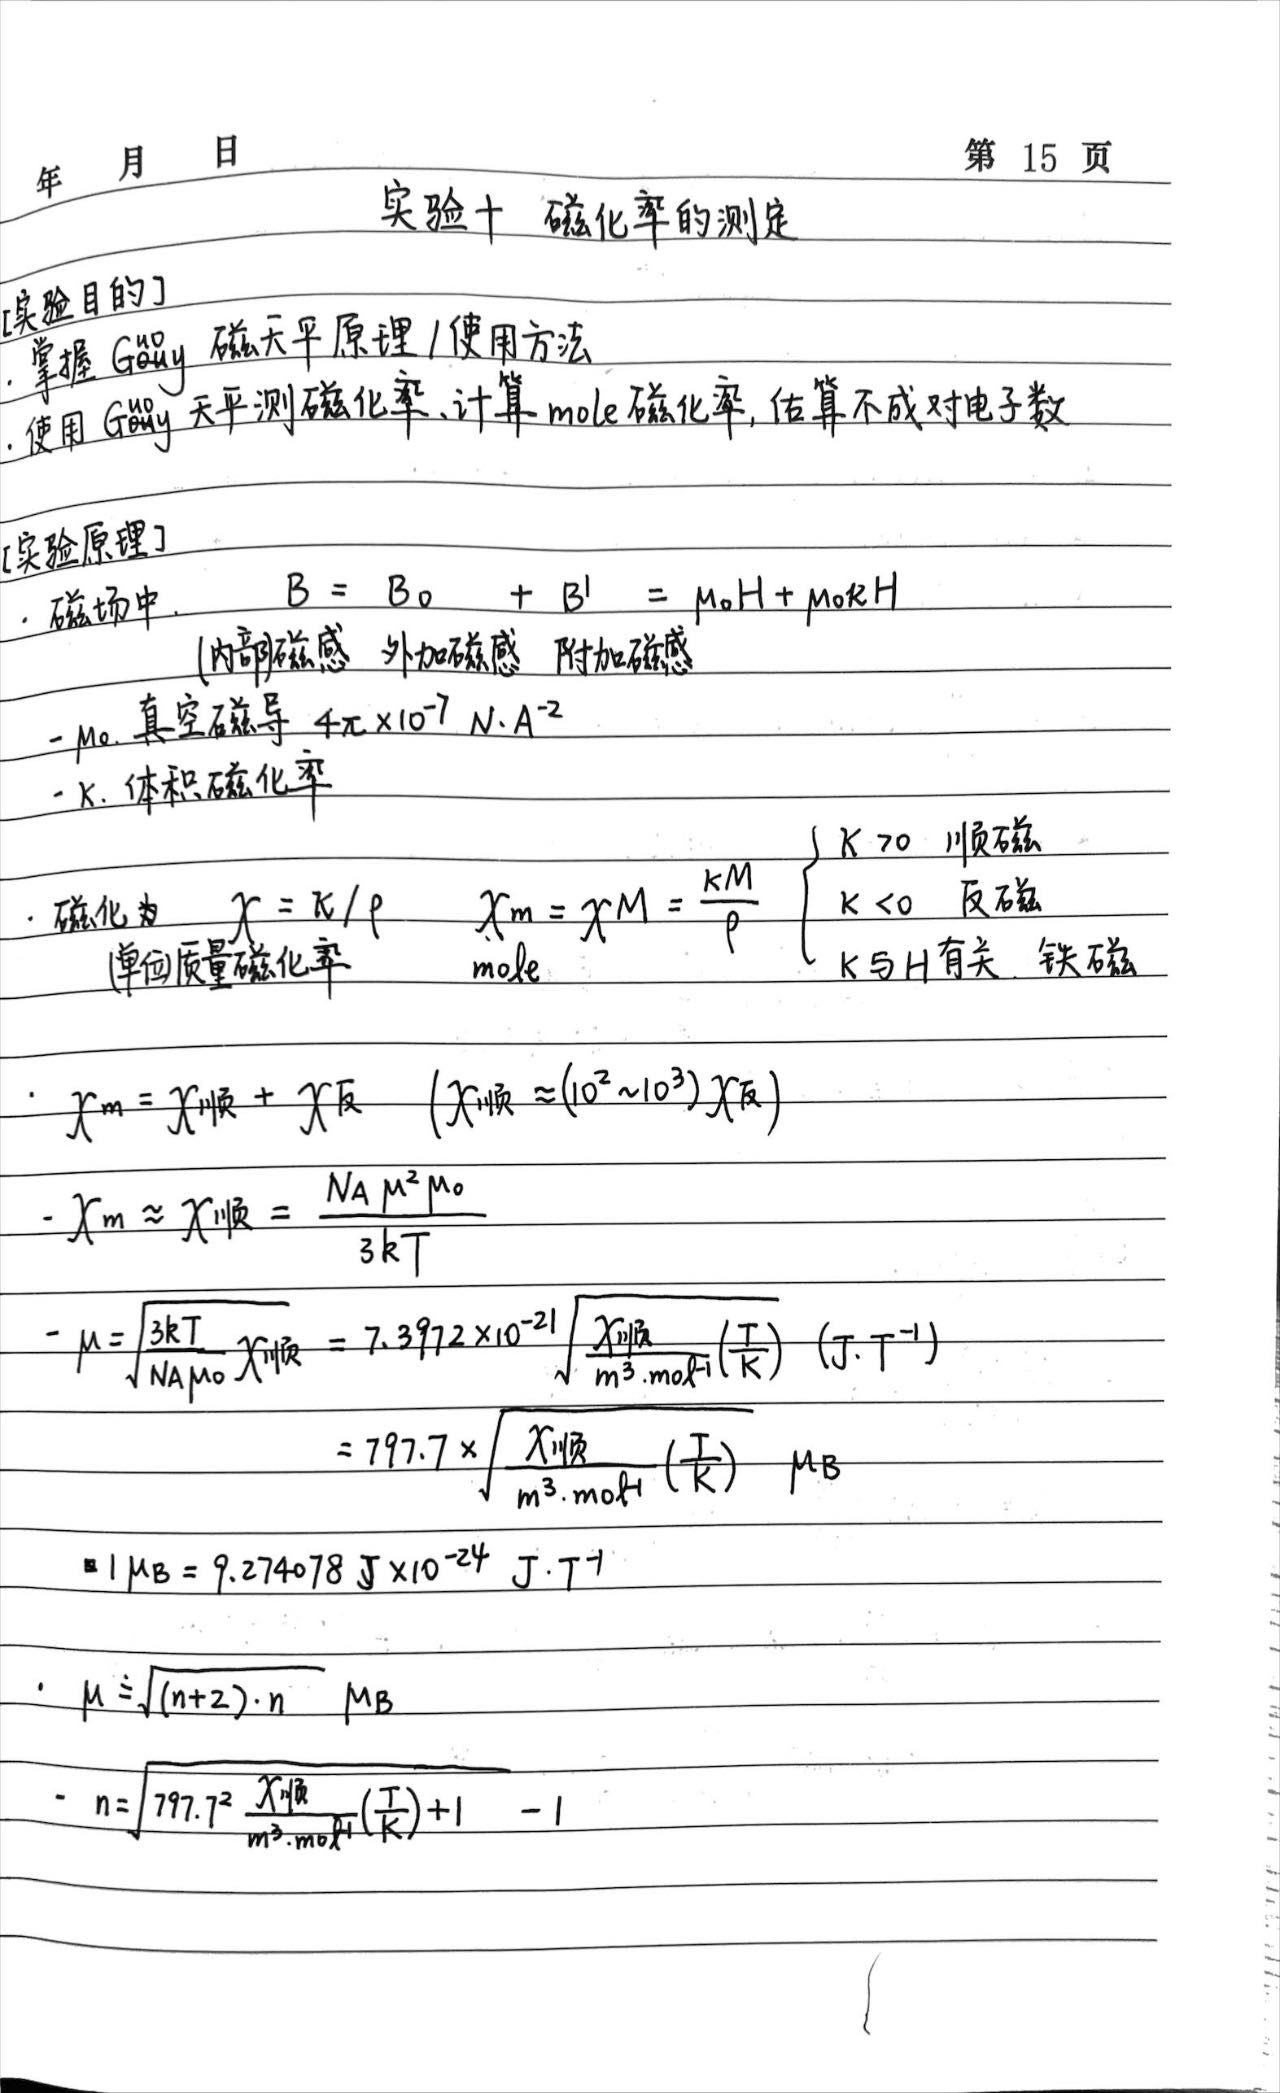
\includegraphics[width=.75\textwidth]{figures/0-1.jpg}
    \caption{预习报告:实验的目的与原理}
\end{figure}
\newpage

\begin{figure}[H]
    \centering
    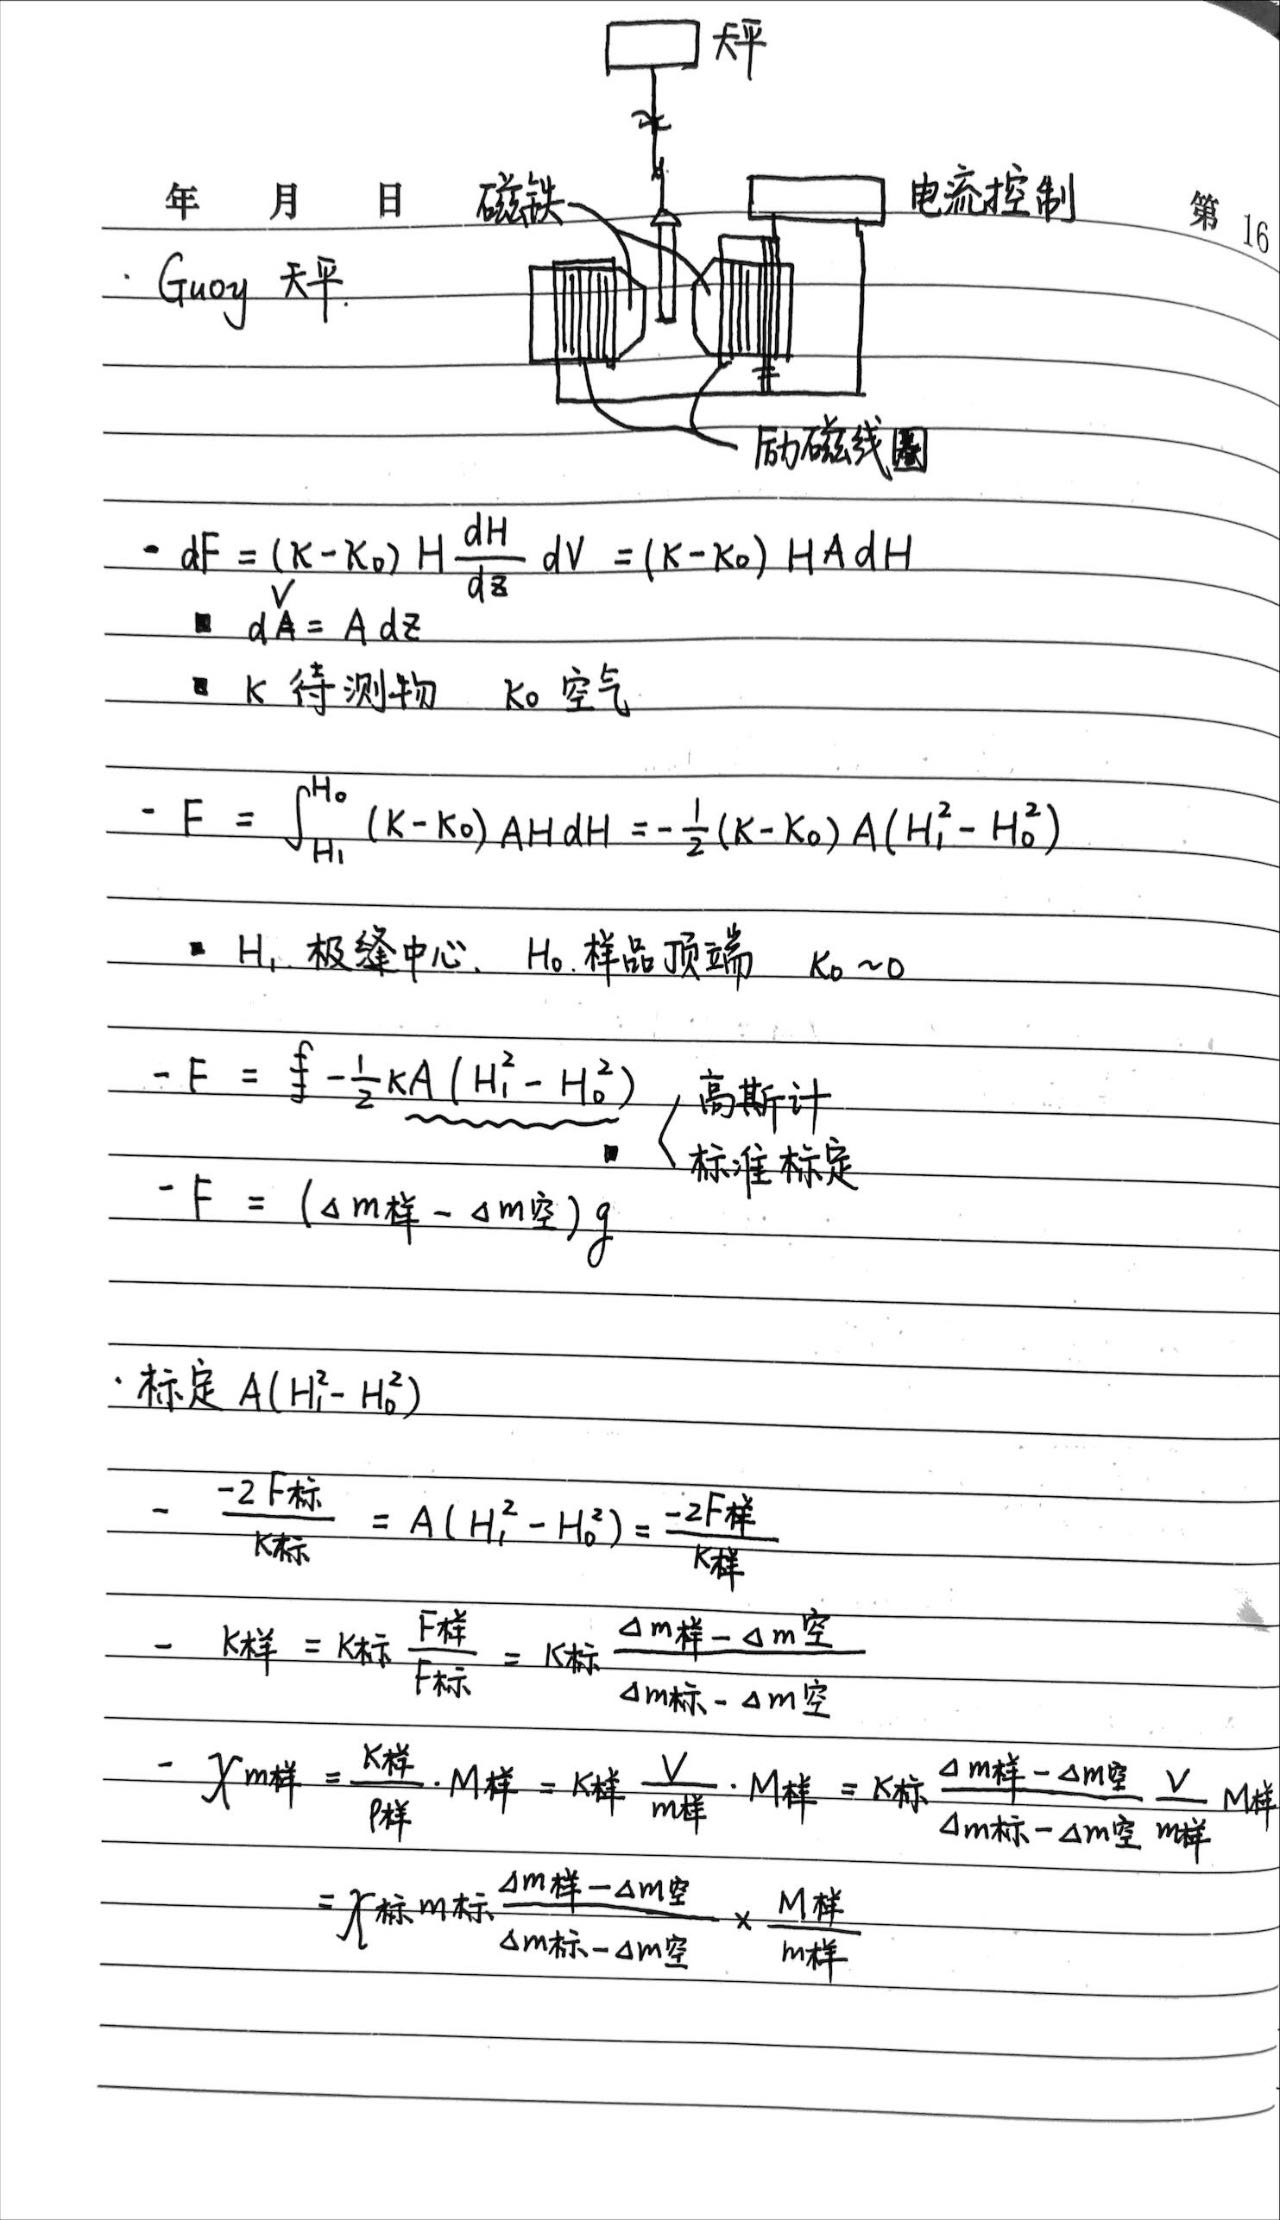
\includegraphics[width=.75\textwidth]{figures/0-2.jpg}
    \caption{预习报告:实验的目的与原理}
\end{figure}
\newpage

\section{实验}

\subsection{仪器、药品、实验步骤与条件}

\begin{figure}[H]
    \centering
    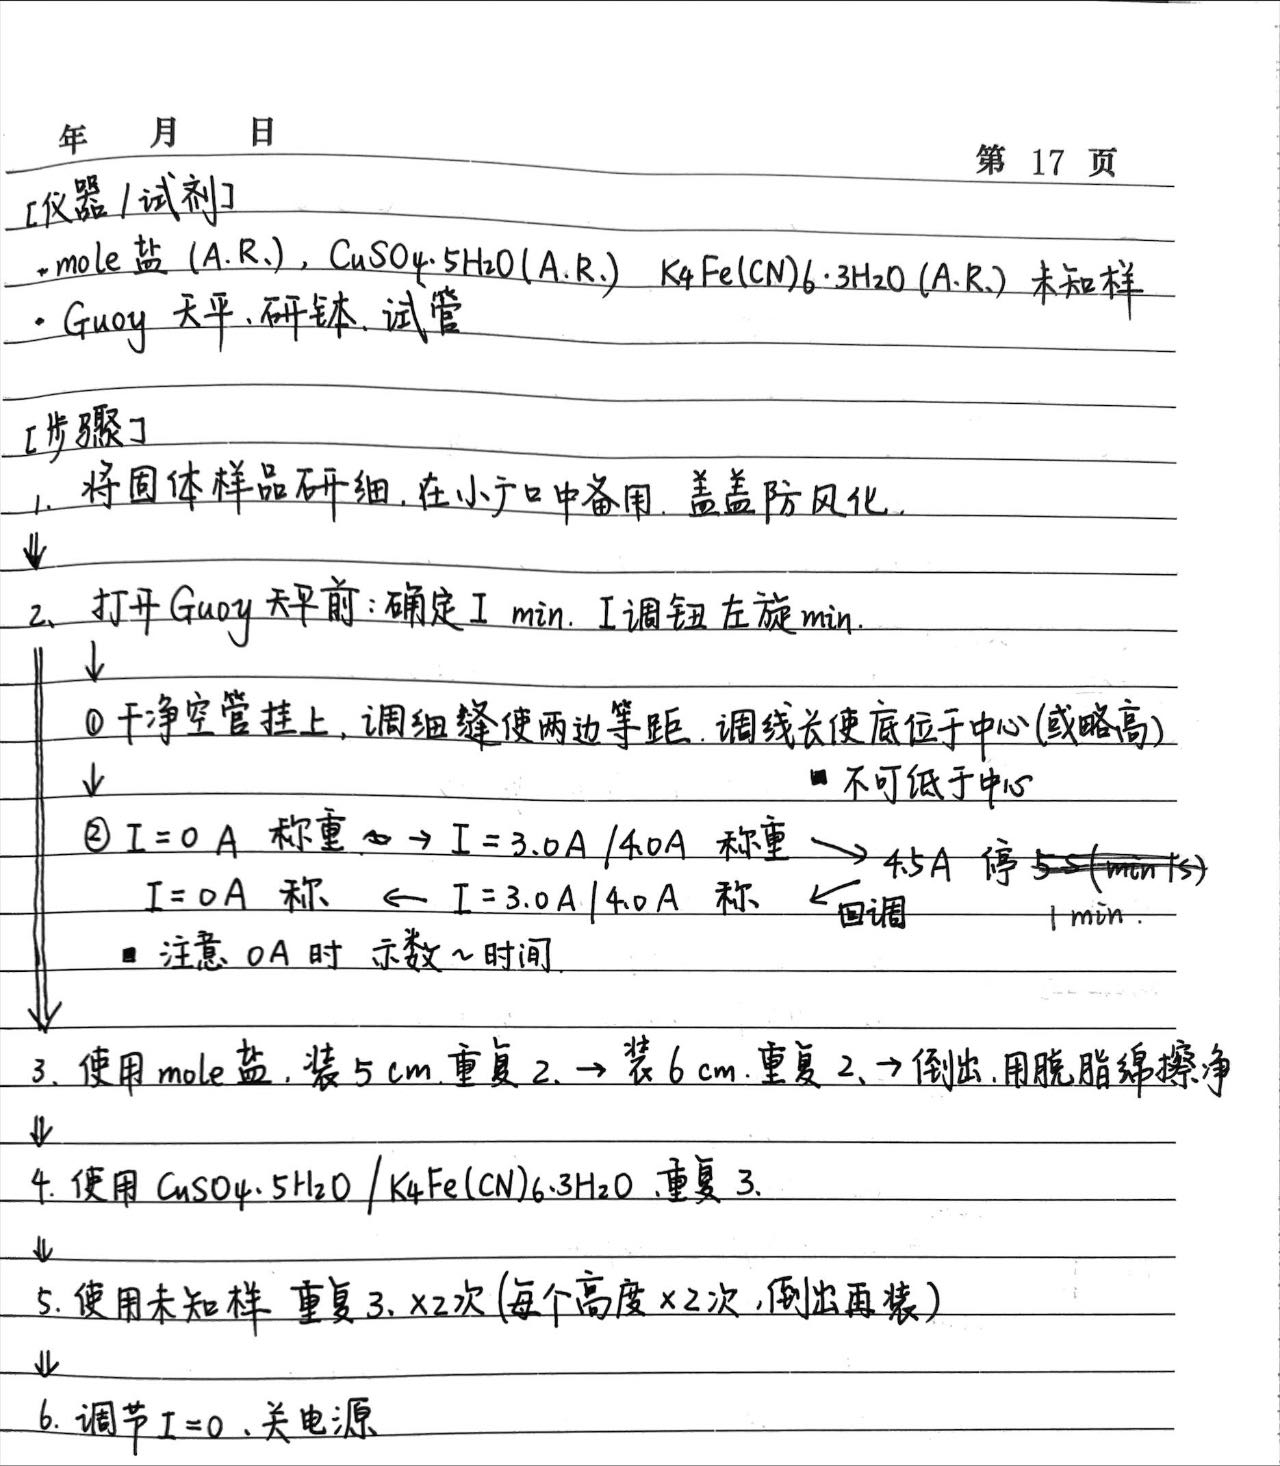
\includegraphics[width=.85\textwidth]{figures/0-3.jpg}
    \caption{预习报告:仪器、药品、实验步骤与条件}
\end{figure}
\newpage





\section{数据处理与结果呈现}

\subsection{实验数据记录}

本实验的原始数据如表 \ref{tab:1}。

\begin{table}[H]
\centering
\caption{实验中测定的磁场强度与其对应的质量}
\begin{tabular}{cccccccccc}
\toprule
\multicolumn{3}{c}{励磁电流/A} & 0 & 3 & 4 & 4.5 & 4 & 3 & 0 \\
\midrule
\multirow{2}{*}{空管} & \multicolumn{2}{c}{$B / \mathrm{mT}$} & 4.7 & 226.4 & 300.5  & / & 301.1 & 227.4 & 4.7  \\
& \multicolumn{2}{c}{$m/ \mathrm{g}$} & 8.5340 & 8.5530 & 8.5320  & / & 8.5322 & 8.5329 & 8.5338 \\
\midrule
\multirow{4}{*}{莫尔盐} & \multirow{2}{*}{$5 \mathrm{~cm}$} & $B / \mathrm{mT}$ & 4.4 & 226.1 & 300.4  & / & 301.0 & 227.0 & 4.5 \\
& & $m/ \mathrm{g}$ & 11.2174 & 11.2575 & 11.2876  & / & 11.2880 & 11.2581 & 11.2174 \\
\cline{2-10}
& \multirow{2}{*}{$6 \mathrm{~cm}$} & $B / \mathrm{mT}$ & 4.4 & 226.2 & 300.6  & / & 301.1 & 227.2 & 4.6 \\
& & $m/ \mathrm{g}$ & 11.7525 & 11.7934 & 11.8243  & / & 11.8248 & 11.7937 & 11.7522 \\
\midrule
\multirow{4}{*}{硫酸铜} & \multirow{2}{*}{$5 \mathrm{~cm}$} & $B / \mathrm{mT}$ & 4.6 & 226.0 & 300.2  & / & 300.9 & 227.1 & 4.3 \\
& & $m/ \mathrm{g}$ & 11.3733 & 11.3803 & 11.3855  & / & 11.3859 & 11.3905 & 11.3731 \\
\cline{2-10}
& \multirow{2}{*}{$6 \mathrm{~cm}$} & $B / \mathrm{mT}$ & 4.2 & 226.1 & 300.3  & / & 301.1 & 227.1 & 4.3 \\
& & $m/ \mathrm{g}$ & 11.8690 & 11.8762 & 11.8819  & / & 11.8820 & 11.8767 & 11.8690 \\
\midrule
\multirow{4}{*}{黄血盐} & \multirow{2}{*}{$5 \mathrm{~cm}$} & $B / \mathrm{mT}$ & 4.3 & 226.1 & 300.6  & / & 301.1 & 227.4 & 4.4 \\
& & $m/ \mathrm{g}$ & 10.9767 & 10.9683 & 10.9669  & / & 10.9673 & 10.9682 & 10.9694 \\
\cline{2-10}
& \multirow{2}{*}{$6 \mathrm{~cm}$} & $B / \mathrm{mT}$ & 4.4 & 225.8 & 300.3  & / & 301.4 & 227.1 & 4.5 \\
& & $m/ \mathrm{g}$ & 11.5262 & 11.5251 & 11.5236  & / & 11.5241 & 11.5251 & 11.5261 \\
\midrule
\multirow{8}{*}{未知样} & \multirow{2}{*}{$5 \mathrm{~cm}$} & $B / \mathrm{mT}$ & 4.2 & 226.0 & 300.3  & / & 301.2 & 227.2 & 4.3 \\
& & $m/ \mathrm{g}$ & 10.9231 & 10.9404 & 10.9529  & / & 10.9533 & 10.9406 & 10.9231 \\
\cline{2-10}
& \multirow{2}{*}{$6 \mathrm{~cm}$} & $B / \mathrm{mT}$ & 4.3 & 226.2 & 300.4  & / & 301.3 & 227.2 & 4.3 \\
& & $m/ \mathrm{g}$ & 11.3090 & 11.3257 & 11.3382  & / & 11.3385 & 11.3257 & 11.3087 \\
\cline{2-10}
& \multirow{2}{*}{$5 \mathrm{~cm}$} & $B / \mathrm{mT}$ & 4.2 & 226.1 & 300.7  & / & 301.3 & 227.1 & 4.3 \\
& & $m/ \mathrm{g}$ & 10.9690 & 10.9865 & 10.9993  & / & 10.9993 & 10.9862 & 10.9689 \\
\cline{2-10}
& \multirow{2}{*}{$6 \mathrm{~cm}$} & $B / \mathrm{mT}$ & 4.2 & 226.0 & 300.5  & / & 301.2 & 227.2 & 4.4 \\
& & $m/ \mathrm{g}$ & 11.3602 & 11.3772 & 11.3905  & / & 11.3905 & 11.3775 & 11.3596 \\

\bottomrule
\end{tabular}
\label{tab:1}
\end{table}

\subsection{莫尔盐的比磁化率}

实验温度$T = 273.15 + 23.2 = 296.4^\circ\mathrm{C}$,根据公式,计算莫尔盐的比磁化率:

\begin{equation*}
    \chi_0=\frac{9500 \times 10^{-9}}{T+1} \times 4 \pi=4.028 \times 10^{-7} \mathrm{~m}^3 \cdot \mathrm{kg}^{-1}
\end{equation*}

\subsection{样品摩尔磁化率与比磁化率的计算}

以励磁电流为$0\mathrm{~A}$时,正向的质量作为基准,考虑空管在不同励磁电流下的质量变化,计算每组实验中样品的质量及其绝对质量变化:
\begin{equation}\label{eq:1}
    \begin{aligned}
        m_a &= m_{a+e} - m_e \\
        \Delta m_a &= (m_a - m_{0\mathrm{A},a}) - (m_e - m_{0\mathrm{A},e})
    \end{aligned}
\end{equation}

根据式 \eqref{eq:1} ,计算得到表 \ref{tab:2}。 

\begin{table}[H]
\centering
\caption{不同条件下样品的绝对质量变化}
\begin{tabular}{cccccccc}
\toprule
样品 & 距离 & $m/ \mathrm{g}$ & $\Delta m_{3\mathrm{A}} / \mathrm{g}$ & $\Delta m_{4\mathrm{A}} / \mathrm{g}$ & $\Delta m_{4\mathrm{A}}^\prime / \mathrm{g}$ & $\Delta m_{3\mathrm{A}}^\prime / \mathrm{g}$ & $\Delta m_{0\mathrm{A}}^\prime / \mathrm{g}$ \\
\midrule
\multicolumn{2}{c}{空管} & 
8.5340 & -0.0010 & -0.0020 & -0.0018 & -0.0011 & -0.0002 \\
\midrule
\multirow{2}{*}{莫尔盐} & $5 \mathrm{~cm}$ & 2.6834 & 0.0411 & 0.0722 & 0.0724 & 0.0418 & 0.0002 \\
& $6 \mathrm{~cm}$ &  3.2185 &  0.0419 &  0.0738 &  0.0741 &  0.0423 & -0.0001 \\
\midrule
\multirow{2}{*}{黄血盐} & $5 \mathrm{~cm}$ &  2.4427 & -0.0004 & -0.0008 & -0.0001 & -0.0006 & -0.0001 \\
& $6 \mathrm{~cm}$ &  2.9922 & -0.0001 & -0.0006 & -0.0003 &  0.0000 &  0.0001 \\
\midrule
\multirow{2}{*}{硫酸铜} & $5 \mathrm{~cm}$ & 2.8393 & 0.0080 & 0.0142 & 0.0144 & 0.0183 & 0.0000 \\
& $6 \mathrm{~cm}$ & 3.3350 & 0.0082 & 0.0149 & 0.0148 & 0.0088 & 0.0002 \\
\midrule
\multirow{4}{*}{未知样} & $5 \mathrm{~cm}$ & 2.3891 & 0.0183 & 0.0318 & 0.0320 & 0.0186 & 0.0002 \\
& $6 \mathrm{~cm}$ & 2.7750 &  0.0177 &  0.0312 &  0.0313 &  0.0178 & -0.0001 \\
& $5 \mathrm{~cm}$ & 2.4350 & 0.0185 & 0.0323 & 0.0321 & 0.0183 & 0.0001 \\
& $6 \mathrm{~cm}$  & 2.8262 &  0.0180 &  0.0323 &  0.0321 &  0.0184 & -0.0004 \\
\bottomrule
\end{tabular}
\label{tab:2}
\end{table}

对于已知化学式的样品:硫酸铜 \ce{CuSO4.5H2O} 与黄血盐 \ce{K4[Fe(CN)6].3H2O},使用公式 \eqref{eq:2} 计算摩尔磁化率,得到表 \ref{tab:3}。
\begin{equation}\label{eq:2}
    \chi_{\mathrm{m},a}=\chi_0 M_a\frac{\Delta m_a}{\Delta m_0} \times \frac{m_0}{m_a}
\end{equation}

对于未知化学式的未知样,使用公式 \eqref{eq:3} 计算其比磁化率,得到表 \ref{tab:4}。
\begin{equation}\label{eq:3}
    \chi_a=\chi_0 \frac{\Delta m_a}{\Delta m_0} \times \frac{m_0}{m_a}
\end{equation}

\begin{table}[H]
    \centering
    \caption{硫酸铜与黄血盐的摩尔磁化率(单位:$10^{-8} \mathrm{~m^3\cdot mol^{-1}}$)}
    \begin{tabular}{cccccc}
        \toprule
        \multicolumn{2}{c}{样品} & $\chi_{3\mathrm{A}}$ & $\chi_{4\mathrm{A}} $ &  $\chi_{4\mathrm{A}}^\prime$ &   $\chi_{3\mathrm{A}}^\prime $\\
        \midrule
        \multirow{2}{*}{硫酸铜} & $5 \mathrm{~cm}$ & 1.850 & 1.869 & 1.891 & 1.887  \\
        & $6 \mathrm{~cm}$ & 1.900 & 1.960 & 1.939 & 2.019  \\
        \midrule
        \multirow{2}{*}{黄血盐} & $5 \mathrm{~cm}$ & -0.4319 & -0.4917 & -0.3678 & -0.4247 \\
        & $6 \mathrm{~cm}$ & -0.1041 & -0.3522 & -0.1754 & 0.000  \\
        \bottomrule
    \end{tabular}
    \label{tab:3}
\end{table}

\begin{table}[H]
    \centering
    \caption{未知样的比磁化率(单位:$10^{-7} \mathrm{~m^3\cdot kg^{-1}}$)}
\begin{tabular}{cccccc}
\toprule
    \multicolumn{2}{c}{样品} & $\chi_{3\mathrm{A}}$ & $\chi_{4\mathrm{A}}$ &  $\chi_{4\mathrm{A}}^\prime$ &   $\chi_{3\mathrm{A}}^\prime$\\ 
    \midrule
    \multirow{4}{*}{未知样} & $5 \mathrm{~cm}$ & 2.028 & 2.006 & 2.014 & 2.027  \\
    & $6 \mathrm{~cm}$ & 1.987 & 1.989 & 1.987 & 1.980  \\
    & $5 \mathrm{~cm}$ & 2.012 & 2.000 & 1.982 & 1.957  \\
    & $6 \mathrm{~cm}$ & 1.984 & 2.022 & 2.001 & 2.009  \\
    \bottomrule
    \end{tabular}
    \label{tab:4}
\end{table}

由于励磁电流下行时,样品会存在剩磁现象;而且根据表 \ref{tab:1} 励磁电流相同时,下行时的磁场会比上行时略强。故本次实验中,只取电流上行时的数据计算最终结果。

分别对2种样品高度,2种励磁电流时的4组数据取平均,得到硫酸铜与黄血盐的摩尔磁化率(根据表 \ref{tab:2},硫酸铜与未知样的$\Delta m$有三位有效数字,黄血盐的$\Delta m$只有一位有效数字):
\begin{align*}
    \bar{\chi}_{\text{m,硫酸铜}} &= 1.90\times 10^{-8} \mathrm{~m^3\cdot mol^{-1}}\\
    \bar{\chi}_{\text{m,黄血盐}} &= -4\times 10^{-9} \mathrm{~m^3\cdot mol^{-1}}
\end{align*}

分别对4种样品高度,2种励磁电流时的8组数据取平均,得到未知样的比磁化率:
\begin{equation*}
    \bar{\chi}_{\text{未知样}} = 2.00\times 10^{-7} \mathrm{~m^3\cdot kg^{-1}}
\end{equation*}

\subsection{样品分子磁矩的计算}

根据公式 \eqref{eq:4},通过摩尔磁化率,计算各个条件下硫酸铜的分子磁矩,得到表 \ref{tab:8}。
\begin{equation}\label{eq:4}
    \mu=797.7 \sqrt{\frac{\chi_m}{\mathrm{~m}^3 \cdot \mathrm{mol}^{-1}}\left(\frac{T}{K}\right)} \mu_B 
\end{equation}

\begin{table}[H]
    \centering
    \caption{硫酸铜的分子磁矩}
    \begin{tabular}{cccccc}
        \toprule
        \multicolumn{2}{c}{样品} & $\mu_{3\mathrm{A}}/\mathrm{\mu_{B}}$ & $\mu_{4\mathrm{A}}/\mathrm{\mu_{B}}$ &  $\mu_{4\mathrm{A}^\prime}/\mathrm{\mu_{B}}$ &   $\mu_{3\mathrm{A}^\prime}/\mathrm{\mu_{B}}$ \\
        \midrule
        \multirow{2}{*}{硫酸铜} & $5 \mathrm{~cm}$ & 1.868 & 1.878 & 1.888 & 1.887  \\
        & $6 \mathrm{~cm}$ & 1.893 & 1.922 & 1.912 & 1.952  \\
        \bottomrule
    \end{tabular}
    \label{tab:8}
\end{table}

对励磁电流上行时的数据取平均,得到:
\begin{equation*}
    \bar{\mu}_{\text{硫酸铜}} = 1.89 \mathrm{~\mu_{B}}
\end{equation*}

\subsection{不成对电子数的计算}

不成对电子书可以由公式 \eqref{eq:5} 计算得到:
\begin{equation}\label{eq:5}
    \mu=\sqrt{n(n+2)} \mu_B
\end{equation}
公式 \eqref{eq:5} 也可以写作一元二次方程形式:
\begin{equation}\label{eq:9}
    n^2 +2n-\mu^2 = 0
\end{equation}
方程 \eqref{eq:9} 的解为:
\begin{equation}\label{eq:10}
    n = \frac{-2+\sqrt{4-4\mu^2}}{2} = \sqrt{1+\mu^2} - 1
\end{equation}

可以求得硫酸铜中单电子数:
\begin{equation*}
n_{\text{硫酸铜}}=\left(\bar{\mu}_{\text{硫酸铜}}^{2} + 1\right)^{0.5} - 1=\left(\left(1.89\right)^{2} + 1\right)^{0.5} - 1=1.14
\end{equation*}

\section{结果与讨论}

% 对自己实验结果可靠性和可信度的论证和评价(如:误差的分析和估算、结果有效数字位数的确定等, 误差分析不要求面面俱到)
\subsection{误差分析}

\subsubsection{莫尔盐比磁化率的不确定度}

假设温度测定的允差为$0.1 ^\circ \mathrm{C}$,由于室温变化导致的误差为$0.2^\circ \mathrm{C}$,故温度测定的误差可以计算得到(为了方便书写,本报告中所有误差的省略单位,其单位与其对应的物理量的单位保持一致):
\begin{equation*}
    \sigma_T = \sqrt{\left(\frac{0.1}{\sqrt{3}}\right)^2+\left(\frac{0.2}{\sqrt{3}}\right)^2} = 0.13 
\end{equation*}

莫尔盐比磁化率的误差:
\begin{equation*}
\begin{aligned}
\frac{\partial \chi_0 }{\partial T }&=- \frac{0.00011938}{\left(T + 1\right)^{2}}=- \frac{0.00011938}{\left(\left(296.35\right) + 1\right)^{2}}=-1.3 \times 10^{-9}\\ 
\end{aligned}
\end{equation*}
\begin{equation*}
\begin{aligned}
\sigma_{\chi_0}&=\sqrt{\left(\frac{\partial \chi_0 }{\partial T } \sigma_{T}\right)^2}\\
&=\sqrt{\left(-1.3 \times 10^{-9} \times 0.13\right)^2}\\
&=\sqrt{\left(-1.8 \times 10^{-10}\right)^2}\\
&=1.8 \times 10^{-10}\ \mathrm{~m^3\cdot mol^{-1}}
\end{aligned}
\end{equation*}

最终,得到莫尔盐比磁化率及其误差:
\begin{equation*}
\chi_0=(4.015  \pm 0.002)\times 10^{-7}\ \mathrm{~m^3\cdot mol^{-1}}
\end{equation*}

\subsubsection{样品摩尔磁化率与比磁化率的不确定度}

假设,本实验中使用的万分之一分析天平的允差为$0.1\mathrm{~mg}$,则考虑其误差:
\begin{equation*}
    \sigma_m = \frac{0.1\times 10^{-3}}{\sqrt{3}} = 5.8\times 10^{-5} 
\end{equation*}
根据公式 \eqref{eq:1},可以得到,质量与质量差的误差:
\begin{align*}
    \sigma_{m_a} &= \sqrt{2}\sigma_m = 8.2\times 10^{-5}\\
    \sigma_{\Delta m_a} &= \sqrt{4}\sigma_m = 1.2\times 10^{-4} 
\end{align*}

根据公式 \eqref{eq:2}、\eqref{eq:3},不妨记:
\begin{equation*}
    r = \frac{\Delta m_a}{\Delta m_0} \times \frac{m_0}{m_a}
\end{equation*}
有:
\begin{equation}\label{eq:6}
\begin{aligned}
    \chi_{\mathrm{m},a} &= \chi_0M_ar_a \\
    \chi_a &= \chi_0r_a 
\end{aligned}
\end{equation}
可得以下公式,求得$r$的误差,得到表 \ref{tab:5}:
\begin{equation*}
\begin{aligned}
    \sigma_r&=|r| \sqrt{\left(\frac{\sigma_{m_0}}{m_0}\right)^2+\left(\frac{\sigma_{m_a}}{m_a}\right)^2+\left(\frac{\sigma_{\Delta m_0}}{\Delta m_0}\right)^2+\left(\frac{\sigma_{\Delta m_a}}{\Delta m_a}\right)^2} \\
\end{aligned}
\end{equation*}

\begin{table}[H]
\centering
\caption{比例系数$r$及其不确定度}
\begin{tabular}{cccccc}
\toprule
样品 & 距离 & $r_{3\mathrm{A}}$ & $r_{4\mathrm{A}}$ & $r_{3\mathrm{A}}^\prime$ & $r_{4\mathrm{A}}^\prime$ \\
\midrule
\multirow{2}{*}{黄血盐} & $5 \mathrm{~cm}$ &  $-0.0088 \pm 0.0027$ & $-0.0101 \pm 0.0015$ & $-0.0075 \pm 0.0015$ & $-0.0087 \pm 0.0026$ \\
& $6 \mathrm{~cm}$ & $-0.0022 \pm 0.0027$ & $-0.0076 \pm 0.0015$ & $-0.0038 \pm 0.0015$ & / \\
\midrule
\multirow{2}{*}{硫酸铜} & $5 \mathrm{~cm}$ & $0.2060 \pm 0.0031$ & $0.2081 \pm 0.0018$ & $0.2105 \pm 0.0018$ & $0.2101 \pm 0.0031$ \\
& $6 \mathrm{~cm}$ & $0.2028 \pm 0.0030$ & $0.2092 \pm 0.0017$ & $0.2070 \pm 0.0017$ & $0.2156 \pm 0.0030$ \\
\midrule
\multirow{4}{*}{未知样} & $5 \mathrm{~cm}$ & $0.3964 \pm 0.0028$ & $0.3921 \pm 0.0016$ & $0.3935 \pm 0.0016$ & $0.3962 \pm 0.0028$ \\
& $6 \mathrm{~cm}$ & $0.3642 \pm 0.0027$ & $0.3645 \pm 0.0015$ & $0.3642 \pm 0.0015$ & $0.3628 \pm 0.0027$ \\
& $5 \mathrm{~cm}$ & $0.4085 \pm 0.0029$ & $0.4060 \pm 0.0017$ & $0.4023 \pm 0.0016$ & $0.3973 \pm 0.0028$ \\
& $6 \mathrm{~cm}$  & $0.3772 \pm 0.0027$ & $0.3843 \pm 0.0016$ & $0.3804 \pm 0.0015$ & $0.3820 \pm 0.0027$ \\
\bottomrule
\end{tabular}
\label{tab:5}
\end{table}

根据公式 \eqref{eq:6},有:
\begin{equation}\label{eq:7}
    \begin{aligned}
        \sigma_{\chi_{\mathrm{m}}}&=M_0 \sqrt{\left(r \sigma_{\chi_0}\right)^2+\left(\chi_0 \sigma_r\right)^2}\\
        \sigma_{\chi}&=\sqrt{\left(r \sigma_{\chi_0}\right)^2+\left(\chi_0 \sigma_r\right)^2}
    \end{aligned}
\end{equation}

根据公式 \eqref{eq:7},可以求得摩尔磁化率与比磁化率的不确定度,如表 \ref{tab:6}、\ref{tab:7}。

\begin{table}[H]
    \centering
    \caption{硫酸铜与黄血盐的摩尔磁化率的不确定度(单位:$10^{-10} \mathrm{~m^3\cdot mol^{-1}}$)}
    \begin{tabular}{cccccc}
        \toprule
        \multicolumn{2}{c}{样品} & $\sigma_{\chi_{3\mathrm{A}}}$ & $\sigma_{\chi_{4\mathrm{A}} }$ &  $\sigma_{\chi_{4\mathrm{A}}^\prime}$ &   $\sigma_{\chi_{3\mathrm{A}}^\prime }$\\
        \midrule
        \multirow{2}{*}{硫酸铜} & $5 \mathrm{~cm}$ & 3.167 & 1.805 & 1.801 & 3.116  \\
        & $6 \mathrm{~cm}$ & 3.043 & 1.731 & 1.723 & 3.021  \\
        \midrule
        \multirow{2}{*}{黄血盐} & $5 \mathrm{~cm}$ & 10.68 & 6.077 & 6.060 & 10.50  \\
        & $6 \mathrm{~cm}$ & 10.72 & 6.089 & 6.064 & /  \\
        \bottomrule
    \end{tabular}
    \label{tab:6}
\end{table}

\begin{table}[H]
    \centering
    \caption{未知样的比磁化率的不确定度(单位:$10^{-10} \mathrm{~m^3\cdot kg^{-1}}$)}
\begin{tabular}{cccccc}
\toprule
    \multicolumn{2}{c}{样品} & $\sigma_{\chi_{3\mathrm{A}}}$ & $\sigma_{\chi_{4\mathrm{A}} }$ &  $\sigma_{\chi_{4\mathrm{A}}^\prime}$ &   $\sigma_{\chi_{3\mathrm{A}}^\prime }$\\
    \midrule
    \multirow{4}{*}{未知样} & $5 \mathrm{~cm}$ & 11.48 & 6.547 & 6.533 & 11.29  \\
    & $6 \mathrm{~cm}$ & 10.82 & 6.162 & 6.137 & 10.71  \\
    & $5 \mathrm{~cm}$ & 11.72 & 6.691 & 6.663 & 11.47  \\
    & $6 \mathrm{~cm}$ & 11.04 & 6.312 & 6.276 & 10.96  \\
    \bottomrule
    \end{tabular}
    \label{tab:7}
\end{table}

对于平均值,可以使用公式 \eqref{eq:8} 计算不确定度:
\begin{equation}\label{eq:8}
    \begin{aligned}
        \sigma_{\bar{\chi_{\mathrm{m}}}}&=\frac{1}{N} \sqrt{\sum_{i=i}^N\left(\sigma_{\chi_{\mathrm{m},i}}\right)^2+s^2} \\
        \sigma_{\bar{\chi}}&=\frac{1}{N} \sqrt{\sum_{i=i}^N\left(\sigma_{\chi_{i}}\right)^2+s^2} \\
    \end{aligned}
\end{equation}

根据 \ref{eq:8} 计算得到:
\begin{align*}
    \sigma_{\bar{\chi}_{\text{m,黄铁盐}}} &= 1.76 \times 10^{-9} \\
    \sigma_{\bar{\chi}_{\text{m,硫酸铜}}} &= 5.10 \times 10^{-10} \\
    \sigma_{\bar{\chi}_{\text{unknown}}} &= 2.61 \times 10^{-9}
\end{align*}

最终,得到各样品(摩尔)比磁化率及其不确定度:
\begin{align*}
    \bar{\chi}_{\text{m,黄血盐}} &= -(4 \pm 2)\times 10^{-9} \mathrm{~m^3\cdot mol^{-1}}\\
    \bar{\chi}_{\text{m,硫酸铜}} &= (1.90 \pm 0.05)\times 10^{-8} \mathrm{~m^3\cdot mol^{-1}}\\
    \bar{\chi}_{\text{未知样}} &= (2.00\pm 0.03)\times 10^{-7} \mathrm{~m^3\cdot kg^{-1}}
\end{align*}

\subsubsection{样品分子磁矩的不确定度}

根据公式 \eqref{eq:4}:
\begin{equation*}
\begin{aligned}
\frac{\partial \bar{\mu}_{\text{硫酸铜}} }{\partial T }&=\frac{398.85 \left(T \bar{\chi}_{\text{m,硫酸
铜}}\right)^{0.5}}{T}=\frac{398.85 \times \left(\left(296.35\right) \times \left(1.895 \times 10^{-8}\right)\right)^{0.5}}{\left(296.35\right)}=0.0032\\
\frac{\partial \bar{\mu}_{\text{硫酸铜}} }{\partial \bar{\chi}_{\text{m,硫酸铜}} }&=\frac{398.85 \left(T \bar{\chi}_{\text{m,硫酸铜}}\right)^{0.5}}{\bar{\chi}_{\text{m,硫酸铜}}}=\frac{398.85 \times \left(\left(296.35\right) \times \left(1.895 \times 10^{-8}\right)\right)^{0.5}}{\left(1.895 \times 10^{-8}\right)}=5.0 \times 10^{7}\\
\end{aligned}
\end{equation*}
\begin{equation*}
\begin{aligned}
\sigma_{\bar{\mu}_{\text{硫酸铜}}}&=\sqrt{\left(\frac{\partial \bar{\mu}_{\text{硫酸铜}} }{\partial T } \sigma_{T}\right)^2+\left(\frac{\partial \bar{\mu}_{\text{硫酸铜}} }{\partial \bar{\chi}_{\text{m,硫酸铜}} } \sigma_{\bar{\chi}_{\text{m,硫酸铜}}}\right)^2}\\
&=\sqrt{\left(0.0032 \times 0.13\right)^2+\left(5.0 \times 10^{7} \times 5.1 \times 10^{-10}\right)^2}\\
&=\sqrt{\left(0.00041\right)^2+\left(0.025\right)^2}\\
&=0.026\ \mathrm{~\mu_{B}}
\end{aligned}
\end{equation*}

最终,得到硫酸铜的分子磁矩及其不确定度:
\begin{equation*}
\bar{\mu}_{\text{硫酸铜}}=\left (1.89 \pm 0.03 \right )\ \mathrm{~\mu_{B}}
\end{equation*}

\subsubsection{单电子数的不确定度}

根据公式 \eqref{10}:
\begin{equation*}
\begin{aligned}
\frac{\partial n_{\text{硫酸铜}} }{\partial \bar{\mu}_{\text{硫酸铜}} }&=\frac{1.0 \bar{\mu}_{\text{硫酸铜}}}{\left(\bar{\mu}_{\text{硫酸铜}}^{2} + 1\right)^{0.5}}=\frac{1.0 \times \left(1.89\right)}{\left(\left(1.89\right)^{2} + 1\right)^{0.5}}=0.88\\
\end{aligned}
\end{equation*}
\begin{equation*}
\begin{aligned}
\sigma_{n_{\text{硫酸铜}}}&=\sqrt{\left(\frac{\partial n_{\text{硫酸铜}} }{\partial \bar{\mu}_{\text{硫酸铜}} } \sigma_{\bar{\mu}_{\text{硫酸铜}}}\right)^2}\\
&=\sqrt{\left(0.88 \times 0.025\right)^2}\\
&=\sqrt{\left(0.022\right)^2}\\
&=0.022
\end{aligned}
\end{equation*}
最终,得到:
\begin{equation}
n_{\text{硫酸铜}}=\left (1.14 \pm 0.02 \right )
\end{equation}
在 \ce{CuSO4.5H2O} 中,$\mathrm{Cu}(\mathrm{II})$ 的 $\mathrm{d}$ 电子排布为 $\left(b_{1 g}\right)^1\left(a_{1 g}\right)^2\left(b_{2 g}\right)^2\left(e_g\right)^4$,$n=1$,这与实验测得的结果基本吻合。

而测得黄血盐为抗磁性,无法通过顺磁性物质的计算公式计算其磁矩与单电子数。低自旋$\mathrm{Fe}(\mathrm{II})$ 的 $\mathrm{d}$ 电子排布为 $\left(t_2g\right)^6\left(e_g\right)^0$,黄血盐并没有单电子,因此 $\chi_{\text{顺}}=0$,$n=0$。

\subsection{结论}

本次实验以莫尔盐作为标准样, 通过古埃磁天平法测得 $23.2^{\circ} \mathrm{C}$ 下五水硫酸铜摩尔比的磁化率为 $(1.90\pm 0.05) \times 10^{-8} \mathrm{~m}^3 \cdot \mathrm{mol}^{-1}$, 文献值\cite{haynes2016crc} 为 $1.835 \times 10^{-8} \mathrm{~m}^3 \cdot \mathrm{mol}^{-1}$,与文献值的偏差为$3.2\%$,可以认为在仪器误差范围内。五水硫酸铜的分子磁矩为 $(1.89\pm 0.03) \mu_B$, 有$(1.14\pm 0.02) \approx 1$个单电子。

三水合黄血盐的摩尔磁化率为 $-(4\pm 2)\times 10^{-9} \mathrm{~m}^3 \cdot \mathrm{mol}^{-1}$,文献值\cite{haynes2016crc} 为 $-2.165 \times 10^{-9} \mathrm{~m}^3 \cdot \mathrm{mol}^{-1}$,与文献值的偏差为$85\%$,但是,由于测定黄血盐时质量变化微小,实验测定的仪器误差与相当大,文献值仍然在实验误差范围内。

未知样品的比磁化率为 $(2.00\pm 0.03) \times 10^{-7} \mathrm{~m^3\cdot kg^{-1}}$ 。

\subsubsection{误差来源}

本实验中的的误差主要来源于:
\begin{enumerate}
    \item \textbf{装样的误差}:实验要求在每次装样时都要确保样品的粗细程度和紧密度保持一致。然而,在实际的操作过程中,这种一致性很难完全达到,从而产生了装样误差。
    \item \textbf{样品管位置的误差}:在实验中,由于悬挂的铜丝并非钢性,可能在装样时受力改变形状,每次悬挂样品管的高度可能会有所不同,这会导致样品管位置的误差。
    \item \textbf{关于磁场强度的误差}:尽管我们在相同的电流条件下进行实验,但磁场强度并不总是完全相同。这意味着即使在相同的电流下,磁场的实际强度仍可能出现微小的变化。
    \item \textbf{磁滞效应导致的误差}:磁滞效应是指在励磁电流逐渐减小时,磁场的读数会偏向于偏大的方向。这种效应在实验中也可能引起误差。  
\end{enumerate}

\subsubsection{测量磁化率的理想条件}

\begin{enumerate}
    \item \textbf{装样的标准化}:尽量采用标准化的方法来装样,确保每次的粗细和紧密度都相似。例如,可以使用特定的工具或模板来帮助进行装样。
    \item \textbf{固定样品管的位置}:使用固定装置或标记来确保样品管每次都被放在相同的位置,从而消除位置误差。
    \item \textbf{稳定的磁场}:确保磁场来源稳定,并使用校准工具定期检查磁场强度。在相同的电流下,磁场强度应该是恒定的。任何偏差都应该被记录并在最后的结果中进行校正。
    \item \textbf{磁滞效应的补偿}:由于磁滞效应可能导致读数偏大,我们可以考虑在测量过程中适当地调整励磁电流,或者使用软磁材料来减少磁滞。
    \item \textbf{环境控制}:确保实验室的温度、湿度和其他可能影响磁场或样品的因素都被控制在一定范围内。
    \item \textbf{经验和技能}:操作者应该受过充分的培训,熟悉所有的操作步骤和潜在的误差来源。
    \item \textbf{校准和复查}:定期使用已知磁化率的标准样品来校准磁天平,并对结果进行复查,以确保测量的准确性。
\end{enumerate}
\subsection{思考题}

\subsubsection*{思考题1}

\begin{enumerate}
    \item \textbf{在相同的励磁电流下,测得的结果仍然会有区别}:根据表 \ref{tab:1},
    \begin{itemize}
        \item 对于两次平行的实验:这是因为仪器在相同励磁电流下,磁场可能会有一定的偏差所致,或者样品管的位置发生变化所致。
        \item 对于装样高度不同的实验:这是因为装样高度的区别导致样品所受磁场不同,或者样品管的位置发生变化所致。
        \item 对于同一组实验:这是因为反向调节励磁电流时,相同电流时磁场强度与正向不同,以及样品的磁滞效应所致。
    \end{itemize}
    \item \textbf{不同励磁电流下的样品磁化率}:
    \begin{itemize}
        \item 根据表 \ref{tab:1},这并没有显著的区别,根据表 \ref{tab:6}、\ref{tab:7},这在实验误差范围内。
    \end{itemize}
\end{enumerate}

\subsubsection*{思考题2}

\begin{enumerate}
    \item \textbf{样品的装填高度及其在磁场中的位置有何要求?}
    
    样品的装填高度应该是一致的,并且为了得到准确的结果,样品需要被放置在磁场的相同位置。最理想的位置是将样品管的底部放置在极缝的中心,以确保样品均匀地受到磁场影响。
    
    \item \textbf{如果样品管的底部不在极缝中心,对测量结果有影响吗?}
    
    如果样品管的底部不在极缝中心,样品会处于一个非均匀的磁场中,这会导致测量的磁化率值偏离真实值。方程 \eqref{eq:11} 不成立。
    \begin{equation}\label{eq:11}
        F = \int_{H_1}^{H_0}(\kappa-\kappa_0)AH\mathrm{d}H=-\frac{1}{2}(\kappa-\kappa_0)A(H_1^2-H_0^2)
    \end{equation}
    
    \item \textbf{装填高度不一致对实验有何影响?}
    
    装填高度的不一致会导致样品的质量与所受磁场的不一致,会导致测量值平行性的偏差,从而导致磁化率的测量结果偏差增大。
    
    \item \textbf{不同装填高度对实验有何影响?}
    
    不同的装填高度意味着样品的质量和体积都会有所不同。如果样品装填高度高,相同质量的样品收到的磁场作用增强,会显现出更强的顺/抗磁性,反之亦然。
\end{enumerate}

\subsubsection*{思考题3}

\begin{enumerate}
    \item \textbf{装样不平行所引入的误差}:当装样不是完全平行时,会导致样品的部分区域受到的磁场强度与其他区域不同,从而引入误差。此误差的大小取决于偏离的程度。越不平行,所引入的误差就可能越大。
    
    \item \textbf{影响本实验结果的主要因素}:主要因素包括装样的高度、样品在磁场中的位置、磁场的均匀性,以及样品装填的平行度。这些因素都会影响到样品所受的磁场强度,进而影响到测量结果。
    
    \item \textbf{如何得到准确的数据}:为了得到准确的数据,需要确保:
    \begin{itemize}
        \item 样品装填高度一致;
        \item 样品管的底部应放在极缝中心,确保样品处于磁场的均匀区域;
        \item 磁场应保持稳定且均匀;
        \item 样品装填应尽量平行,避免引入不必要的误差。
    \end{itemize}
\end{enumerate}

\subsection{意见与建议}
\begin{enumerate}
    \item \textbf{实验仪器的改进}:
    \begin{itemize}
        \item 使用更加现代化的古埃磁天平,例如将电子天平与磁线圈一体化,而非由两个独立的仪器拼接得到:两个仪器拼接并不紧密,中间会有一小段暴露的区域,会导致铜线受气流影响而摆动,影响实验测量。
        \item 将用于悬挂样品的铜丝改为更加粗和坚固的铜线,以避免其发生形变影响实验结果的一致性。
    \end{itemize}
    \item \textbf{实验方法的改进}:
    \begin{itemize}
        \item 使用更加先进的装样方法,保证每次装样的一致性,例如第一次装样后,第二次装样的质量要与第一次的质量保持完全一致,在质量和高度两个维度都要保持一致性。
        \item 实验的平行性实际取决于磁场强度而非励磁电流的大小,因此,更科学的方法应当是保持每组实验间的磁场强度一致,而不仅仅是励磁电流一致。
    \end{itemize}
\end{enumerate}

\nocite{*}
\bibliography{reference}

\newpage
\section*{附录}
\begin{figure}[H]
    \centering
    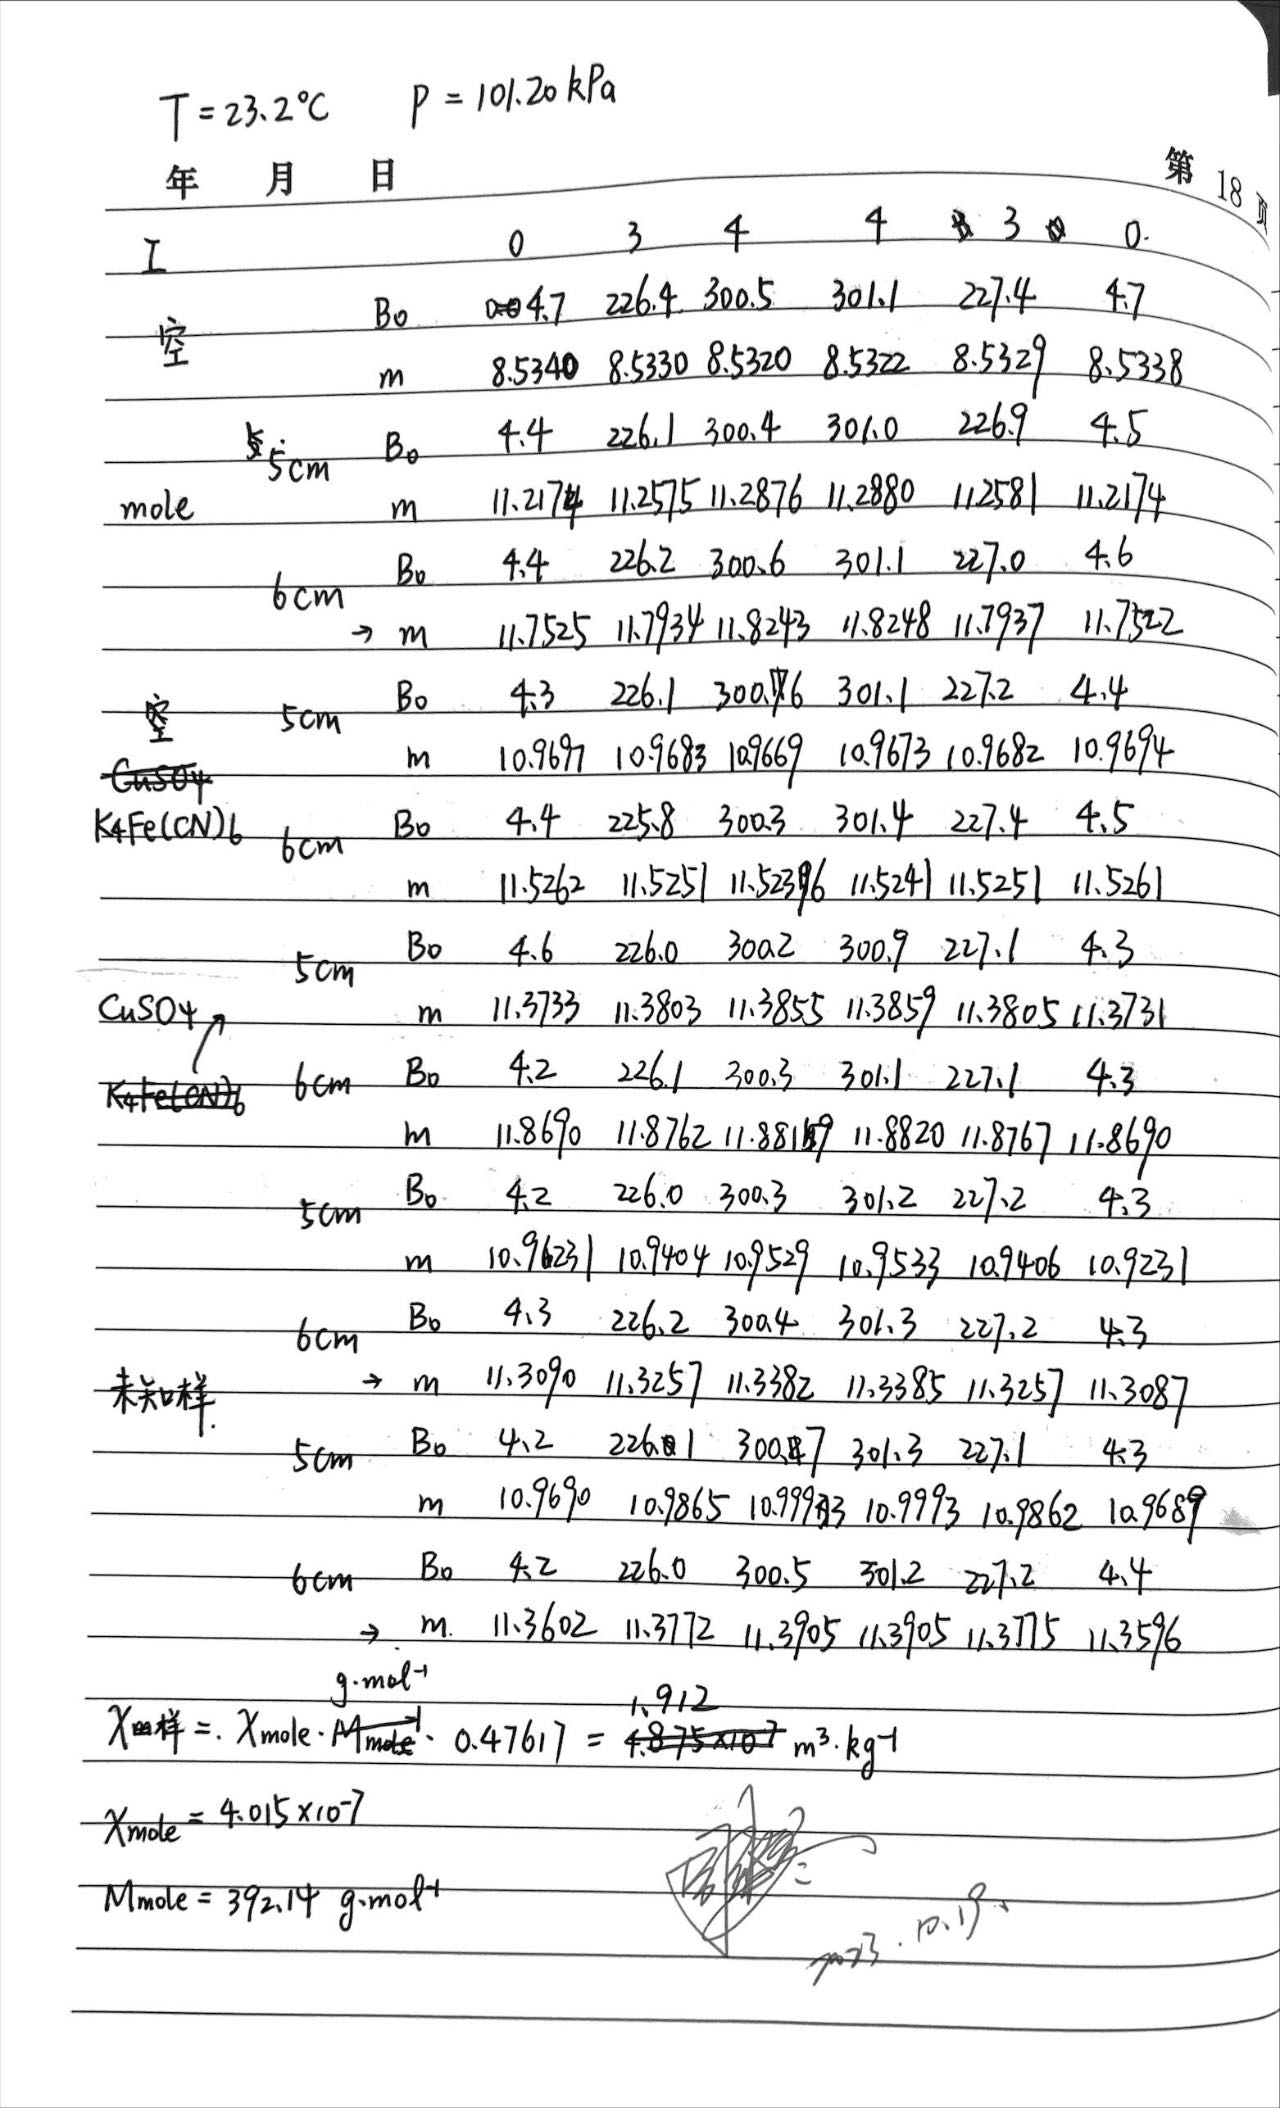
\includegraphics[width=.7\textwidth]{figures/0-4.jpg}
    \caption*{实验报告:原始数据记录}
\end{figure}

\end{document}
